

\documentclass{article}
\usepackage[spanish]{babel}
\usepackage{graphicx}
\usepackage{listings}
\setlength{\parindent}{0pt}
\setlength{\parskip}{3mm}
\usepackage[numbers]{natbib}
\usepackage{color}
\usepackage{url}
%\usepackage{indentfirst} for APA margins and French indention

%-------------------------------------------------------------------------------
% Configuring customized document margins
%-------------------------------------------------------------------------------
\usepackage{geometry}
%\addtolength{\oddsidemargin}{-.75in}
%\addtolength{\evensidemargin}{-.75in}
%\addtolength{\textwidth}{1.4in}
%
%\addtolength{\topmargin}{-0.25in}
%\addtolength{\textheight}{1.65in}

\definecolor{mygreen}{rgb}{0,0.6,0}
\definecolor{mygray}{rgb}{0.5,0.5,0.5}
\definecolor{mymauve}{rgb}{0.58,0,0.82}
\lstset{ 
  backgroundcolor=\color{white},   % choose the background color; you must add \usepackage{color} or \usepackage{xcolor}; should come as last argument
  basicstyle=\footnotesize,        % the size of the fonts that are used for the code
  breakatwhitespace=false,         % sets if automatic breaks should only happen at whitespace
  breaklines=true,                 % sets automatic line breaking
  captionpos=b,                    % sets the caption-position to bottom
  commentstyle=\color{mygreen},    % comment style
  deletekeywords={...},            % if you want to delete keywords from the given language
  escapeinside={\%}{)},          % if you want to add LaTeX within your code
  extendedchars=true,              % lets you use non-ASCII characters; for 8-bits encodings only, does not work with UTF-8
  firstnumber=1,                % start line enumeration with line 1000
  frame=single,	                   % adds a frame around the code
  keepspaces=true,                 % keeps spaces in text, useful for keeping indentation of code (possibly needs columns=flexible)
  keywordstyle=\color{blue},       % keyword style
  language=Octave,                 % the language of the code
  morekeywords={*,...},            % if you want to add more keywords to the set
  numbers=left,                    % where to put the line-numbers; possible values are (none, left, right)
  numbersep=5pt,                   % how far the line-numbers are from the code
  numberstyle=\tiny\color{mygray}, % the style that is used for the line-numbers
  rulecolor=\color{black},         % if not set, the frame-color may be changed on line-breaks within not-black text (e.g. comments (green here))
  showspaces=false,                % show spaces everywhere adding particular underscores; it overrides 'showstringspaces'
  showstringspaces=false,          % underline spaces within strings only
  showtabs=false,                  % show tabs within strings adding particular underscores
  stepnumber=1,                    % the step between two line-numbers. If it's 1, each line will be numbered
  stringstyle=\color{mymauve},     % string literal style
  tabsize=2,	                   % sets default tabsize to 2 spaces
  title=\lstname                  % show the filename of files included with \lstinputlisting; also try caption instead of title
}



\begin{document}

\title{Tarea No.2: Rectificada}
\author{Dayli Machado (5275)}
\date{\today}
\maketitle



\section{Grafo simple no dirigido acíclico usando \textit{bipartite layout}}

Un grafo simple no dirigido acíclico, es aquel que no posee dirección en sus aristas, ni bucles, y no es reflexivo \cite{Elisa}. Este tipo de grafos suele representarse por una secuencia de nodos unidos por aristas, donde de cada nodo generalmente solo sale o llega una arista \cite{Net}. 

Este tipo de grafos puede emplearse para representar estructuras moleculares que sigan este comportamiento, un ejemplo sería la representación de alcanos de tipo lineal, donde los átomos se representan por los nodos y los enlaces entre estos por las aristas. El tipo de algoritmo de acomodamiento (\textit{layout}) que se utilizó para lograr esta representación fue el \textit{bipartite layout} el cual permite posicionar los nodos en dos líneas rectas y trazar ejes entre ellos \cite{layout}, a partir de tener dos conjuntos de nodos diferentes se puede graficar la relación entre ellos. Se observa en la línea de código número 28 la forma de representar esta función empleada para la representación del grafo. Ver figura \ref{fig:Fig01} en la página \pageref{fig:Fig01}.

\newpage
\lstinputlisting[language=Python]{grafo1laybi.py}

\begin{figure}[htbp]
    \centering
    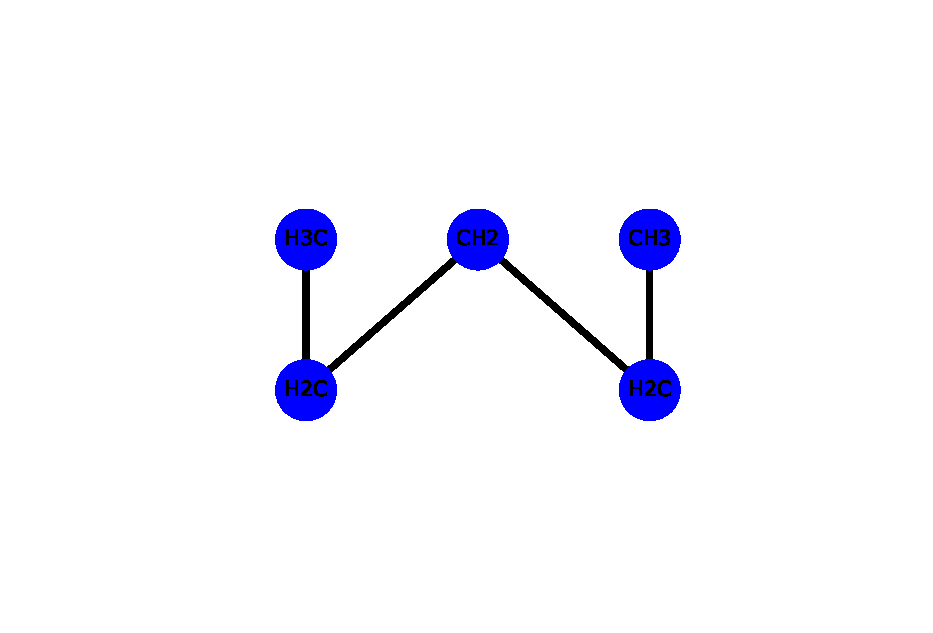
\includegraphics[scale=0.4]{imagenes1/Fig01.eps}
    \caption{Molécula de alcano lineal usando \textit{bipartite layout}}
    \label{fig:Fig01}
\end{figure}

\section{Grafo simple no dirigido cíclico usando \textit{circular layout}}

Un grafo simple no dirigido cíclico es aquel que no posee dirección en sus aristas, pero si se forma un ciclo que represente una figura cerrada que comience y termine en el mismo vértice, entonces es llamado cíclico \cite{redes}. En los grafos no dirigidos el flujo puede fluir en ambas direcciones.

Este tipo de grafos suele representarse por una secuencia de nodos unidos por aristas, pero estos pueden tener dentro un ciclo, o ser un ciclo en sí mismo. En la práctica pudiera ser la representación de las autopistas de una región dada, o también la representación de otro tipo de moléculas de alcanos que posean áreas cerradas en su representación, o las llamdas que se realizan interdepartamentales en una empresa.

Se toma de ejemplo las llamadas que se realizan entre los departamentos de producción, de marketing, comercial, calidad y planificación de la producción en una empresa, donde cada nodo representa un departamento y las aristas las llamadas que se realizan entre ellos. Para este tipo de grafo se emplea el \textit{layout circular} como algoritmo de acomodamiento, pues permite ubicar los nodos en círculos \cite{layout}. De esta forma se visualiza mejor la distribución espacial de los nodos y la relación entre ellos que son las llamadas, pero como en este ejemplo la posición de los nodos puede ser aleatoria, se puede emplear también el \textit{ramdom layout} como otro algoritmo de acomodamiento pues este permite ubicar los nodos uniformemente al azar en el cuadro \cite{layout}. En la figura \ref{fig:Fig02} en la página \pageref{fig:Fig02} se muestra la representación gráfica del mismo.

\newpage
\lstinputlisting[language=Python]{grafo2laycir.py}

\begin{figure}[htbp]
    \centering
    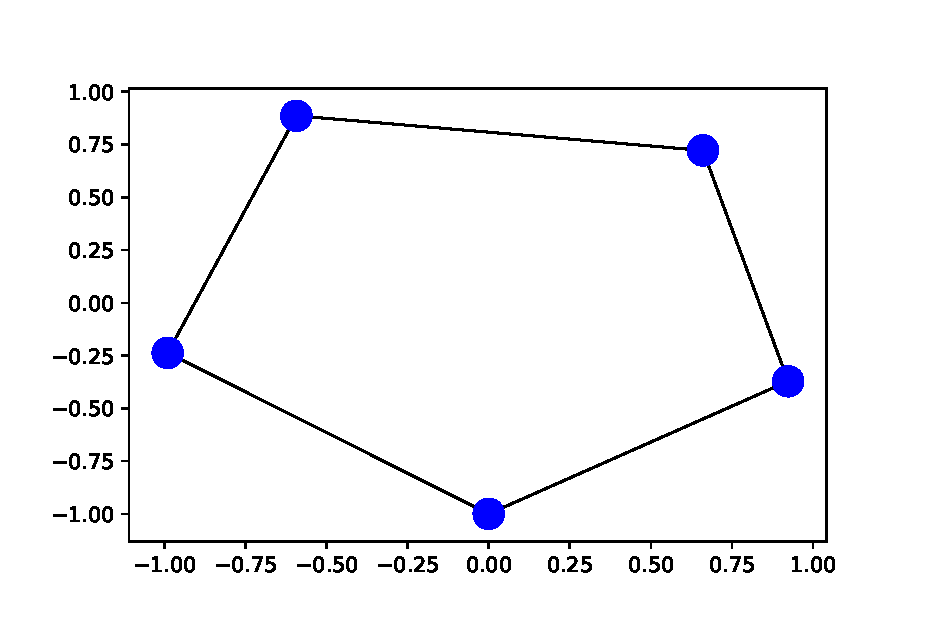
\includegraphics[scale=0.4]{imagenes1/Fig02.eps}
    \caption{Llamadas interdepartamentales usando acomodo circular}
    \label{fig:Fig02}
\end{figure}

\section{Grafo simple no dirigido reflexivo usando \textit{circular layout}}

Un grafo simple no dirigido reflexivo es aquel en el cual no se permiten aristas múltiples, no posee dirección en sus aristas y cuenta al menos con un bucle, lo que se refiere a una arista reflexiva en la que coinciden el vértice de origen y el de destino \cite{Elisa}. 

Este grafo puede emplearse para representar el entrecruzamiento de grupos raciales, donde cada grupo representa un nodo diferente y las relaciones entre los grupos seran los hijos que tengan, siendo una relación no dirigida. Al relacionarse entre la misma raza estarían ocurriendo lazos reflexivos. Si se consideran los cuatro grupos representativos de las razas humanas según la clasificación de especialistas serían: blanco/caucásico, asiático/mongoloide, negroide/negro y australoide; esta clasificación posee dentro de cada grupo una clasificación de hasta 30 subgrupos, pero solo se representarán los cuatro principales. El \textit{layout} que mejor refleja este tipo de grafo es el circular, la justificación es la misma explicada en la sección anterior. El código para representar este grafo fue tomado y adaptado del sitio \cite{codimag}, el mismo permitió insertar las imágenes como nodos. Ver figura \ref{fig:Fig03} en la página \pageref{fig:Fig03}.
\newpage
\lstinputlisting[language=Python]{grafo3laycir.py}

\begin{figure}[htbp]
    \centering
    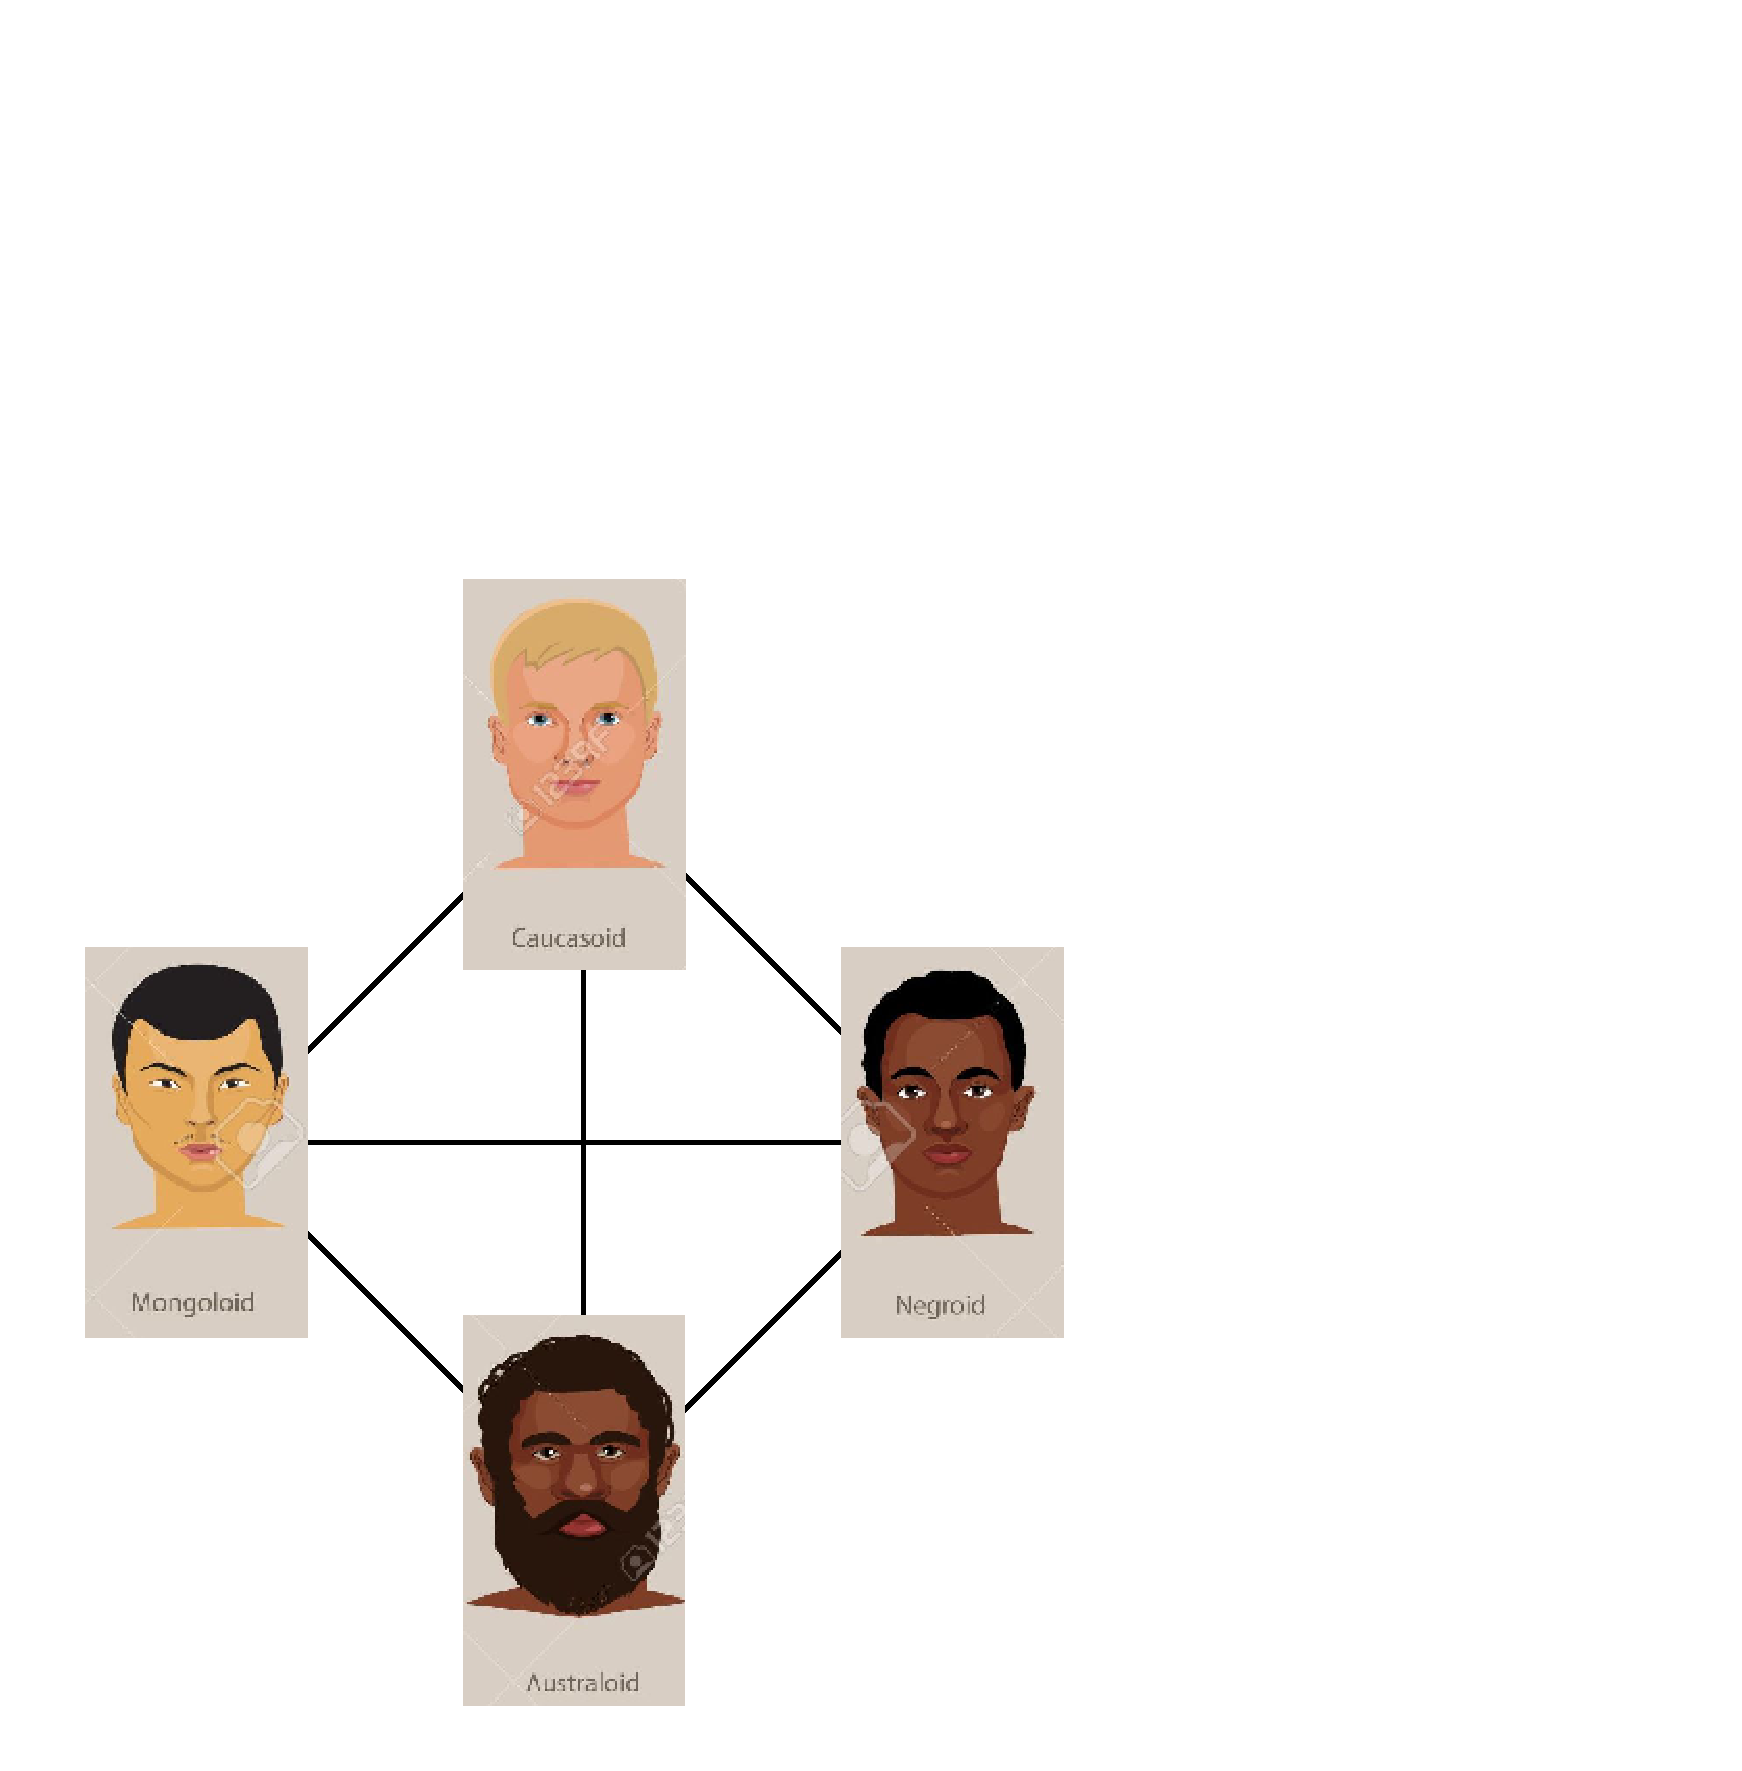
\includegraphics[scale=0.4]{imagenes1/Fig03.eps}
    \caption{Grupos raciales usando \textit{circular layout}}
    \label{fig:Fig03}
\end{figure}

\section{Gráfo simple dirigido acíclico usando \textit{spring layout}}

Un grafo simple dirigido acíclico, es aquel que posee una dirección en sus aristas, y no posee bucles o reflexividad, ni ciclos \cite{Elisa}.
 
En este caso, ejemplos de la vida real son aquellos que poseen un origen del que puede salir una o varias aristas por diferentes caminos sin que entre ellas existan ciclos y posean un destino final diferente al del origen. 

Los árboles genealógicos, los organigramas en las empresas, el flujo de procesos industriales que no posean ciclos, con un inicio y un fin, pudieran resultar ser ejemplos de la vida real en los que se puede aplicar este tipo de grafos. 

Como algoritmo de acomodo para representar este grafo se usó el \textit{spring layout}, el cual permite representar de manera sencilla las aristas rectas que salen de un nodo a otro y fijar la posición haciendo uso de sus parámetros \cite{layout} siendo el mismo algoritmo empleado en la tarea anterior para este tipo de grafo, sin embargo en este ejercicio se profundizó en el uso de sus parámetros. 

Para la representación inicial se fija la posición de los nodos y el centro del grafo, además se estableció una distancia estándar entre ellos, también se emplea el degradado de color para indicar la transformación que recibe un objeto dado en una línea de producción. Ver figura \ref{fig:Fig04} en la página \pageref{fig:Fig04}.

\newpage
\lstinputlisting[language=Python]{grafo4lyspring.py}

\begin{figure}[htbp]
    \centering
    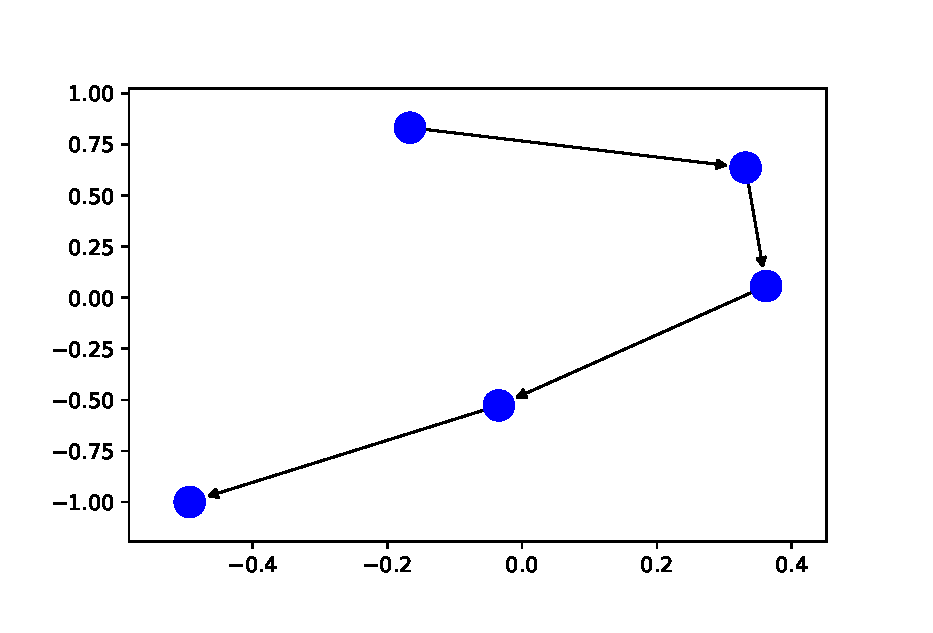
\includegraphics[scale=0.6]{imagenes1/Fig04.eps}
    \caption{Transformación de un objeto en una línea de producción usando \textit{spring layout} }
    \label{fig:Fig04}
\end{figure}


\section{Gráfo simple dirigido cíclico usando \textit{bipartite layout} }

Un grafo simple dirigido cíclico es aquel que posee una dirección en sus aristas y una figura cerrada que comienza y  termina en el mismo vértice.

Para este caso ejemplos de la vida real son aquellos que poseen un origen del que puede salir una o varias aristas por diferentes caminos, y que en un determinado nodo regresan a alguno anterior de modo que se forme uno o más ciclos. El destino final suele ser diferente al del origen. 

Como aplicación real de este tipo de grafo se explica el flujo de procesos industriales o artesanales que posean ciclos, por ejemplo: la elaboración artesanal de jugo de naranja, al representar este proceso en un flujograma mediante un diagrama OPERIN, en el que se reflejen sus operaciones. Una vez que se llegue al paso de exprimir las naranjas, se cae en un ciclo volviendo a la operación anterior de seleccionar otra y otra naranja hasta cubrir toda la capacidad del extractor de jugo. En esta segunda tarea el algoritmo de acomodo empleado que se usó para representarlo fue el \textit{bipartite layout} pues resulta más sencillo y directo para graficar los nodos que salen de la línea de producción y que forman el ciclo con los que se mantienen en ella, se emplea el parámetro \textit{top} para separar el conjunto de nodos que no están en la línea principal de producción. Con este algoritmo se aprecia una mejor representación del grafo, aunque es válido aclarar que este ejemplo no se comporta exactamente como un grafo bipartito, pero este fue el algoritmo de acomodo que mejor lo representó. En este ejemplo las operaciones son los nodos  y los enlaces la transformación que va teniendo la naranja como se muestra en la figura \ref{fig:Fig05} en la página \pageref{fig:Fig05}.

\newpage
\lstinputlisting[language=Python]{grafo5laybi.py}

\begin{figure}[htbp]
    \centering
    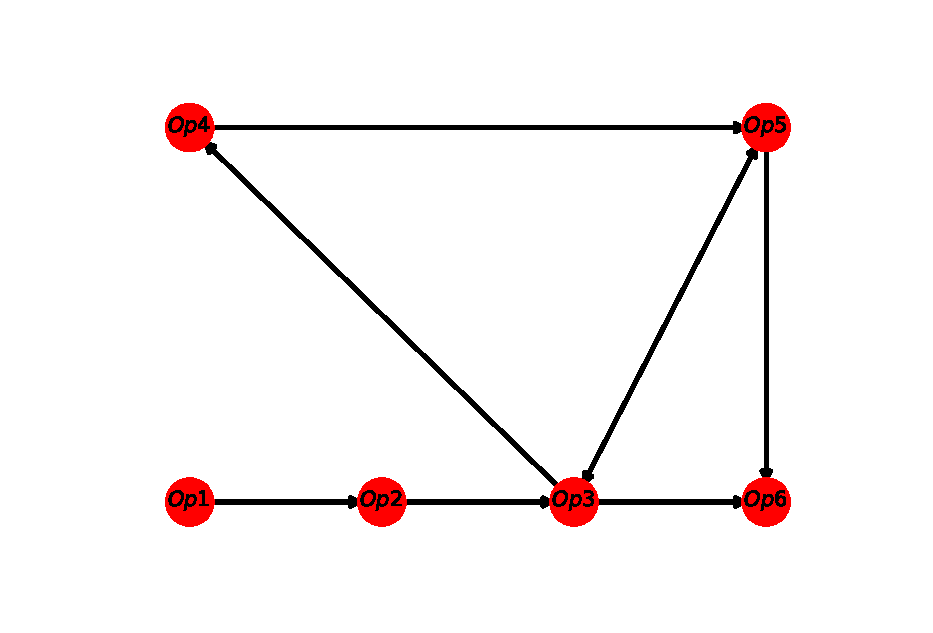
\includegraphics[scale=0.6]{imagenes1/Fig05.eps}
    \caption{Flujo cíclico de una línea de producción artesanal de jugo de naranja}
    \label{fig:Fig05}
\end{figure}

\section{Gráfo simple dirigido reflexivo usando \textit{circular layout}}

La diferencia con este grafo y el anterior reflexivo visto, es que en este caso las aristas sí tienen sentido y el flujo que se analice debe ir en una dirección. En este caso deberá existir un nodo que se llame a sí mismo, o sea, que posea al menos un bucle.

Un ejemplo en el que se puede emplear la teoría de grafos de este tipo es para representar la disposición  de personas con grupos sanguíneos diferentes a recibir sangre compatible o no. La reflexividad está dada en los casos en que cada grupo sanguíneo puede recibir de otros grupos y de sí mismo, excepto el grupo O- que sólo puede recibir del mismo tipo. Se cambia el algoritmo de acomodo anterior por el \textit{circular layout} haciendo uso de sus parámetros, y se evidencia más estabilidad en las iteraciones de la figura que mantienen la misma posición deseada cada vez que se itera, sin tener que entrarla manualmente.
Este se muestra en la figura \ref{fig:Fig06} en la página \pageref{fig:Fig06}.

\newpage
\lstinputlisting[language=Python]{grafo6laycir.py}

\begin{figure}[htbp]
    \centering
    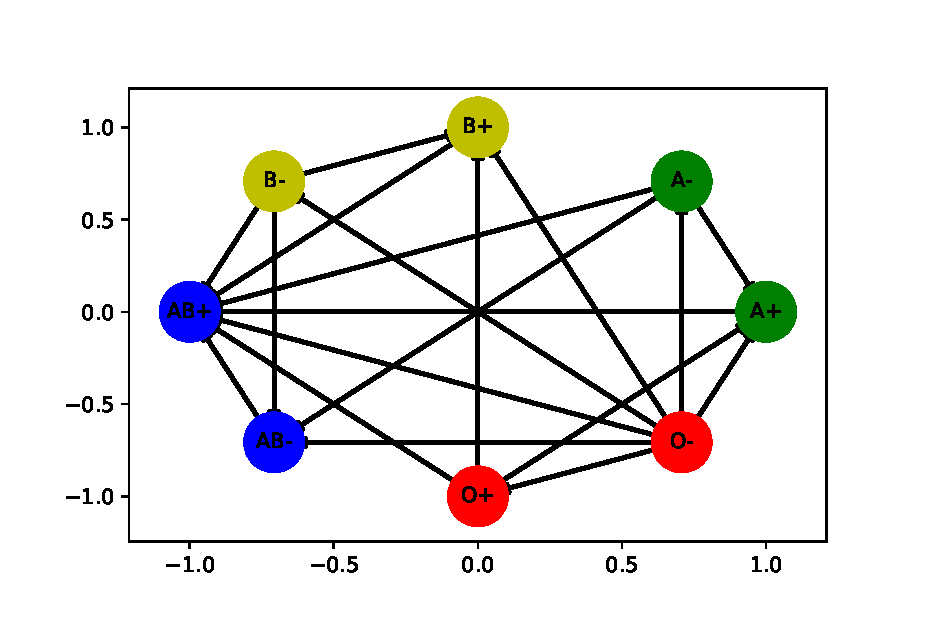
\includegraphics[scale=0.6]{imagenes1/Fig06.eps}
    \caption{Compatibilidad entre grupos sanguíneos}
    \label{fig:Fig06}
\end{figure}

\section{Multigrafo no dirigido acíclico usando \textit{spring layout}}

Un multigrafo no dirigido acíclico es cuando existe más de una arista entre un par de vértices. Si no se permiten aristas múltiples, el grafo es simple \cite{Elisa}. Será no dirigido cuando las aristas no posean sentido restringido, sino que el flujo fluye en ambas direcciones, y en este caso no presenta ciclos.

Un ejemplo práctico de multígrafo no dirigido acíclico es la representación de determinados enlaces moleculares, como por ejemplo: un enlace de doble éster, como es el caso del éster sulfúrico. Para la representación de los elementos con este tipo de grafo se puede emplear el algoritmo de acomodo \textit{spring layout}, es el mismo que se usó en el caso anterior pero esta vez se hace uso de sus parámetros sin fijar la posición \cite{layout}, de este modo se obtiene una representación más ajustada a la realidad, también pudiera emplearse el \textit{Kamada Kawai layout} pero al compararlos e iterar el \textit{spring layaut} devuelve variantes más atractivas. El grafo usando \textit{spring layout} se muestra en la figura \ref{fig:Fig07} en la página \pageref{fig:Fig07}.

\newpage
\lstinputlisting[language=Python]{grafo7lyspring.py}

\begin{figure}[htbp]
    \centering
    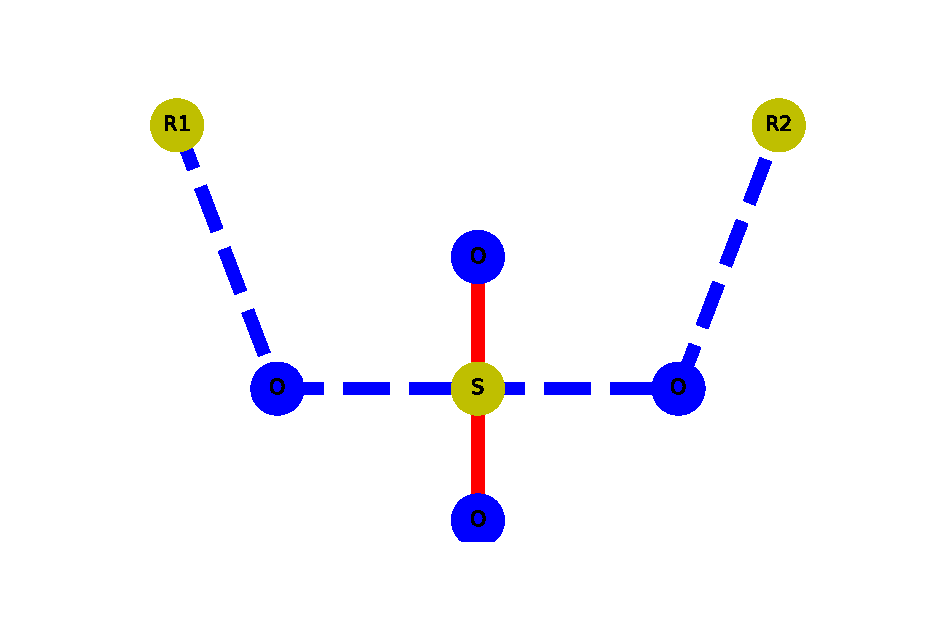
\includegraphics[scale=0.4]{imagenes1/Fig07.eps}
    \caption{Mólecula de éster sulfúrio}
    \label{fig:Fig07}
\end{figure}

\section{Multigrafo no dirigido cíclico usando \textit{Kamada Kawai layout}}

Cuando exista más de una arista entre un par de vértices, el grafo se llama multígrafo. En este caso será no dirigido cuando las aristas no poseen sentido restringido, sino que el flujo fluye en ambas direcciones, y deberán existir zonas cerradas, o sea, que regresen al vértice inicial.

Este tipo de grafo es de gran utilidad para representar el comportamiento de redes sociales y neuronales \cite{redes}. 
El ejemplo práctico mostrado es cuando tenemos necesidad de comunicarnos con alguien por las vías de comunicación que tenemos en la actualidad, donde cada vía de comunicación seleccionada tendrá un costo (peso), y existen muchas vías para comunicarnos con otras personas, y a su vez para otras personas se comuniquen con nosotros, por lo que no es dirigido, pero sí cíclico, debido a los lazos que se pueden formar entre las personas que necesitan comunicarse. El algoritmo de acomodo empleado para este ejemplo según sus prestaciones fue el \textit{Kamada Kawai layout} pues este tiene en cuenta para la representación el peso de la longitud del camino \cite{layout} y devuelve grafos más atractivos para el ejemplo en cuestión. El ejemplo se restringe a solo dos vías de comunicación, ya sea por \textit{whatsap}, o por llamadas telefónicas, aunque en la práctica existen muchas más. Este grafo se muestra en la figura \ref{fig:Fig08} en la página \pageref{fig:Fig08}. 
\newpage
\lstinputlisting[language=Python]{grafo8lykk.py}

\begin{figure}[htbp]
    \centering
    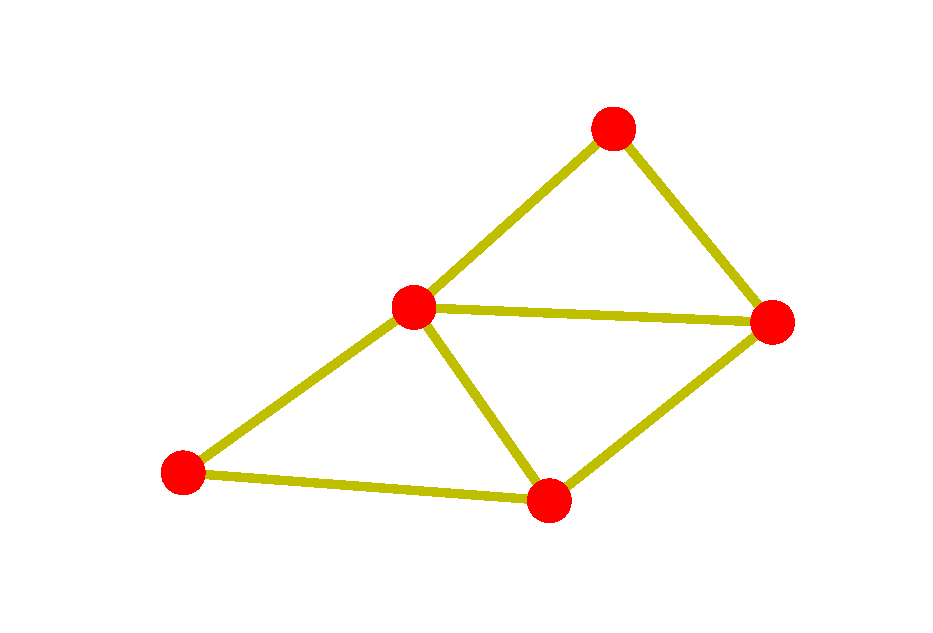
\includegraphics[scale=0.6]{imagenes1/Fig08.eps}
    \caption{Vías de comunicación entre las personas}
    \label{fig:Fig08}
\end{figure}

\section{Multigrafo no dirigido reflexivo usando \textit{random layout}}

Este caso se refiere a un multígrafo en el que existe más de una arista entre un par de vértices, sin dirección entre estas, pero de un nodo deben salir más de una arista que regresen al mismo nodo, sin pasar por otro.

Una aplicación pudiera ser la relación que existe entre cinco signos zodiacales, donde cada nodo representa a las personas de un signo determinado y de cada uno de ellos puede salir una arista que represente las relaciones positivas entre los diferentes signos y otra las relaciones negativas, y a su vez las personas del mismo signo se relacionarán con sus iguales de manera positiva o negativa, lo que representa la reflexibilidad. Este es un grafo que no es exigente para su representación y aunque un algoritmo de acomodo circular puede ser apropiado, se propone usar uno aleatorio que funciona igual en este ejemplo y consume menos. Este grafo se muestra para cinco signos cualesquiera del zodiaco en la figura \ref{fig:Fig09} en la página \pageref{fig:Fig09}. 

\newpage
\lstinputlisting[language=Python]{grafo9lyrandom.py}

\begin{figure}[htbp]
    \centering
    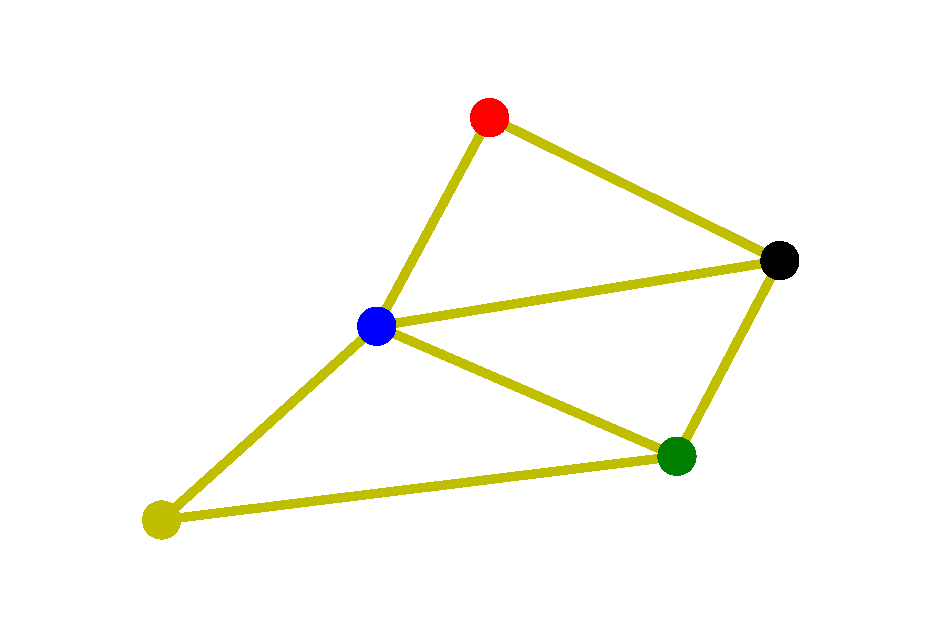
\includegraphics[scale=0.6]{imagenes1/Fig09.eps}
    \caption{Relación entre personas del mismo signo zodiacal}
    \label{fig:Fig09}
\end{figure}

\section{Multigrafo dirigido acíclico usando \textit{spectral layout}}

Para definir un multigrafo dirigido acíclico debe existir más de una arista entre un par de nodos, con dirección y no formar ninguna figura cerrada dentro del grafo. 

Este ejemplo aplicado a la práctica puede ser la representación de un viajero que desea ir de una ciudad a otra para visitarlas y tiene que elegir entre varias rutas posibles para llegar, o pudiera elegir también entre diferentes medios de transporte para trasladarse entre las ciudades, o una combinación de ambos. En este caso las ciudades serían los nodos, y las rutas o medios de transporte posibles a elegir entre un nodo u otro serían las aristas. Una ruta pudiera ser ir de la ciudad de Matanzas en Cuba, a la Habana, de esta a Monterrey, de Monterrey a Torreón y de ahí a Sinaloa. Para devolver el acomodo de estos  nodos puede emplearse el algoritmo \textit{spectral layout} que no se ha empleado en las secciones anteriores, este devuelve una forma sinusoidal pues refleja el algoritmo basado en la utilización de los vectores del gráfico laplaciano \citep{layout}, lo cual no afecta a la visualización del grafo ejemplo. Asimismo se puede emplear el \textit{Kamada Kawai layout} con resultados gráficos más direccionados y apropiados para el ejemplo, pero ya se usó en secciones anteriores. El grafo se muestra en la figura \ref{fig:Fig10} en la página \pageref{fig:Fig10}. 

\lstinputlisting[language=Python]{grafo10lyspectral.py}

\begin{figure}[htbp]
    \centering
    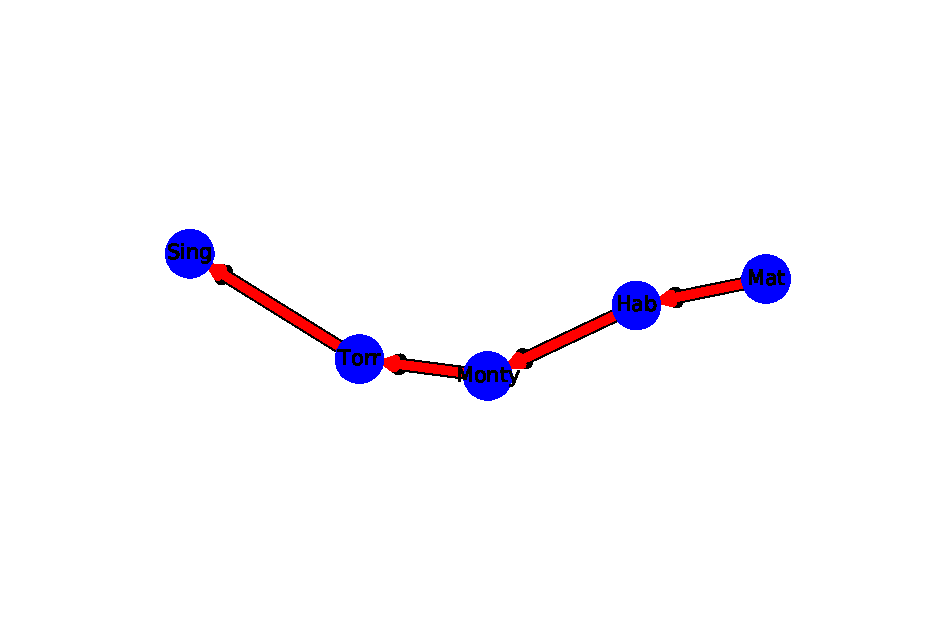
\includegraphics[scale=0.6]{imagenes1/Fig10.eps}
    \caption{Ruta para viajar de Matanzas a Sinaloa}
    \label{fig:Fig10}
\end{figure}

\section{Multigrafo dirigido cíclico usando \textit{spring layout}}

En este tipo de grafos dirigidos cíclicos debe existir más de una arista entre un par de nodos, con dirección y además formarse al menos una figura cerrada dentro del grafo. 

Un ejemplo que representa este tipo de grafo sería la representación del flujo que siguen los pacientes una vez que asisten a la consulta de cuerpo de guardia del ISSSTE, en la que las operaciones del proceso serían los nodos y la clasificación del tipo de paciente y su recorrido dentro de la instalación las aristas. En este caso el cliente al llegar pasa por la consulta de clasificación y ahí le asignan un color en función de la gravedad de su dolencia, se asumen tres colores, rojo, amarillo y verde, que van de mayor gravedad a menor respectivamente y de esta dependerá el tiempo de espera para pasar a la siguiente consulta donde se encuentra el doctor, existe tres consultas con doctores disponibles y de ahí pueden pasar al laboratorio, u a otras de las salas. Luego, del laboratorio pueden pasar nuevamente a la consulta del doctor para revisar los resultados y ocurriría un ciclo, o del doctor directo a la sala, luego al laboratorio y retornar nuevamente al doctor, y ocurriría otro ciclo. El algoritmo de acomodo que mejor se ajustó fue el \textit{spring layout}. Este grafo se muestra en la figura \ref{fig:Fig11} en la página \pageref{fig:Fig11} donde se muestra la representación gráfica del mismo. 
\newpage
\lstinputlisting[language=Python]{grafo11lyspring.py}

\begin{figure}[htbp]
    \centering
    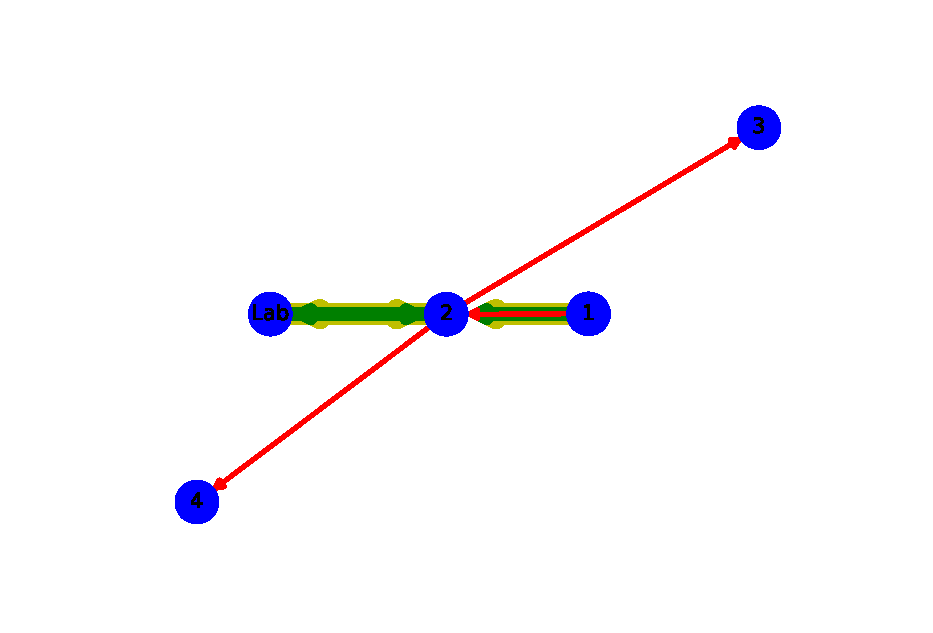
\includegraphics[scale=0.6]{imagenes1/Fig11.eps}
    \caption{Recorrido del paciente en la sala de urgencias del ISSSTE}
    \label{fig:Fig11}
\end{figure}

\section{Multigrafo dirigido reflexivo usando \textit{shell layout} } 

En los multigrafos dirigidos debe existir más de una arista entre un par de nodos, con dirección y además cada nodo debe llamarse a sí mismo.

Un ejemplo en el que el empleo de la teoría de grafos como los que se analizan en esta sección puede emplearse es en el estudio de la influencia de la religión en la sociedad, como un subejemplo de la aplicación en redes sociales.\cite{redes}. 
Por ejemplo, si cada nodo es una persona religiosa creyente, ese nodo (persona) constantemente se realiza un autoexamen de conciencia a sí mismo, evaluando cómo ha sido su actitud con respecto a las variables a analizar en este autoexamen. Estas variables pueden ser operacionalizadas como cada una de las doctrinas de cada religión, las cuales varían de una religión a otra, pero son más de una y pueden agruparse por categorías. Estas variables representan las aristas, cada una puede tener un peso determinado según sea el interés del estudio, a su vez estas mismas doctrinas (convertidas en variable) serán las que cada persona creyente se encargará de transmitir a otras personas creyentes o no, pudiera decirse que se transmite el tipo de actitud que se debe tener ante cada una de estas variables de una persona a otra. En este ejemplo se puede evaluar el impacto en un grupo poblacional que puede tener un tipo de creencia u otro en la medida en que aumente la red. Para este ejemplo se reservó el algoritmo de acomodamiento \textit{shell layout} es un algoritmo que acomoda los nodos en círculos concéntricos \cite{layout} este transmite la idea de expansión que es justamente lo que se desea reflejar en el ejemplo propuesto, si se llevara a gran escala. Una simplificación de este tipo de grafo se representa en la figura \ref{fig:Fig12} en la página \pageref{fig:Fig12}.
\newpage

\lstinputlisting[language=Python]{12rectificado.py}
\newpage
\begin{figure}[htbp]
    \centering
    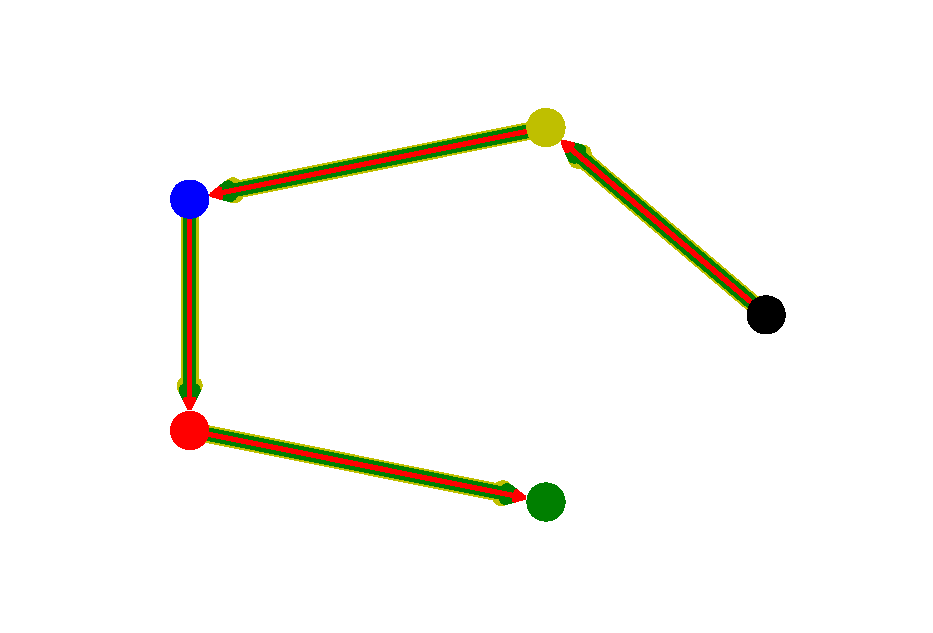
\includegraphics[scale=0.6]{imagenes1/Fig12.eps}
    \caption{Expansión de doctrinas religiosas}
    \label{fig:Fig12}
\end{figure}

\newpage
\bibliography{Referencias_1}
\bibliographystyle{plainnat}
\end{document}